\documentclass{mywork}
\addtolength{\headheight}{\baselineskip}
\lhead{Hauptseminar\\ \today}
\chead{komplexe dynamische Systeme}
\rhead{\theauthor}
\renewcommand{\theta}{\vartheta}
\newcommand{\D}{\mathbb{D}}
\cfoot[LE,RO]{\bfseries\color{gray} -~\thepage~-}
\usepackage{pgfplots}
\begin{document}

\section{Motivation: das Newton-Verfahren}

Die Newtoniteration ist gegeben durch die Abbildung
\[
	\Phi(x)=z-\frac{f(z)}{f'(z)}
\]
Dabei ist für einen Startwert $z_0$ folgendes Verhalten denkbar
\begin{itemize}
\item Das Newton-Verfahren konvergiert gegen eine Nullstelle von $f$
\item Das Newton-Verfahren konvergiert nicht.
\end{itemize}

Das Newton-Verfahren konvergiert lokal. Wie ist das Konvergenzverhalten außerhalb dieser Konvergenzumgebung?

$\longrightarrow$ Newton-Fraktale.


\begin{figure}[H]
\centering
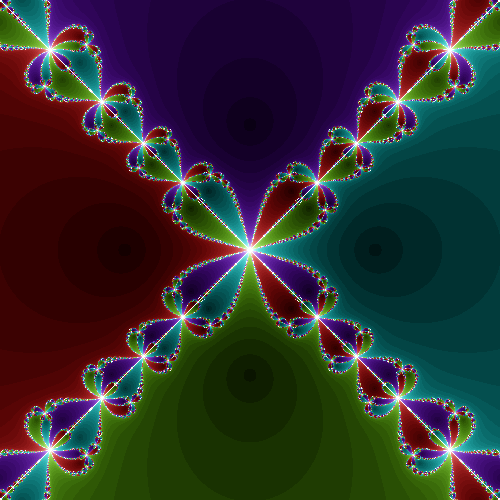
\includegraphics[scale=0.3]{fraktal.png}
\caption{Newton-Fraktal für $f(z)=z^4-1$}
\end{figure}


Dies motiviert das Konzept der \emph{Fatou-} bzw. \emph{Juliamenge}:
\begin{description}
\item[Fatou-Menge] Die Startwerte aus dieser Menge führen unter Iteration zu einer ,,stetigen`` Dynamik, das heißt, eine kleine Änderung des Startwert führt zu einer ähnlichen Dynamik.
\item[Julia-Menge] Beschreibt die Menge der Startpunkte, die zu den ,,instabilen`` Prozessen gehören. Jede noch so kleine Änderung des Startwerts führt zu einer komplett anderen Dynamik.
\end{description} 
Notation: $F(f)$ bezeichnet die Fatoumenge von $f$ und $J(f)$ analog die Juliamenge von $f$.


\section{Allgemeine Definitionen}

\begin{df} \label{1}
Sei $z_0$ periodischer Punkt bzgl. $f$ mit Periode n, d.h. $f^n(z_0)=z_0$. Dann heißt er
\begin{itemize}
\item \emph{stark anziehend}, falls $|(f^n)'(z_0)|=0$,
\item \emph{anziehend}, falls $0<|(f^n)'(z_0)|<1$,
\item \emph{indifferent}, wenn $|(f^n)'(z_0)|=1$,
\item \emph{abstoßend}, wenn $|(f^n)'(z_0)|>1$.
\end{itemize} 
\end{df}


\begin{df}[Einzugsgebiet] \label{2}
Ist $z_0$ ein anziehender periodischer Punkt von $f$, dann ist die Menge
\[
	A(z_0)=\{z\in \overline{\mathbb{C}}: \lim\limits_{L\ni k\to \infty} f^k(z)=z_0, L\subset \N\}
\]
das \emph{Einzugsgebiet} (engl. \emph{basin of attraction}) von $z_0$.
\end{df}



\begin{df}[Julia-Menge] \label{3}
Wir definieren die Julia-Menge durch
\[
J(f):=\overline{\{z\in \overline{\mathbb{C}}: z \text{ abstossender periodischer Punkt von $f$} \}}
\]
Und die Fatou-Menge durch $F(f)=J(f)^c$
\end{df}


\section{Normale Familien und exzeptionelle Punkte}

\begin{df} \label{4}
Eine Familie $\{F_n\}$ analytischer Funktionen operiert \emph{normal} auf $U$, falls jede Folge $(F_{n_i})_{i\in \mathbb{N}}$ eine Teilfolge $(F_{n_{i_j}})_{j\in \N}$ besitzt, sodass einer der beiden Eigenschaften erfüllt ist:
\begin{itemize}
\item $F_{n_{i_j}}$ konvergiert gleichmäßig auf kompakten Mengen $K\subset U$.
\item $F_{n_{i_j}}$ divergiert gleichmäßig gegen $\infty$ auf $U$.
\end{itemize}
Eine Familie $\{F_n\}$ analytischer Funktionen operiert \emph{nicht normal} bei $z_0$, falls er in keiner Umgebung \emph{normal} operiert.
\end{df}



\begin{ex}\label{5}
Betrachte die Funktion $F$, gegeben durch $F(x)=ax$. Definiere die Familie $\{F^n\}$.

\textbf{Fall 1: $|a|<1$.} so konvergiert für jede kompakte Teilmenge die Funktionenfolge $F^n(z)=a^n\cdot z$ gleichmäßig gegen 0. 

$\longrightarrow F(f)=\bar{\mathbb{C}}$, $A(0)=\C$, $A(\infty)=\{\infty\}$.

\textbf{Fall 2: $|a|>1$.} Die Familie $\{F\}$ operiert nicht normal bei $0$, denn für $z\neq 0$ divergiert jede beliebige Teilfolge.

$\longrightarrow J(F)=\{0\}$, $A(0)=\{0\}$, $A(\infty)=\bar{\C}\setminus \{0\}$. 
\end{ex}



\begin{prop}\label{6}
Sei $F$ analytisch, $z_0$ ein abstoßender periodischer Punkt bzgl. $F$. Dann operiert die Familie $\{F^n\}_{n\in \N}$ nicht normal bei $z_0$.
\end{prop}
\begin{proof}[Für Fixpunkte]
 Angenommen $\{F^n\}$ operiert normal auf einer Umgebung $U$ von $z_0$. Da für alle $n\in \N$ $F^n(z_0)=z_0$, folgt insbesondere, dass $F^n$ nicht (gleichmäßig) gegen $\infty$ auf $U$ divergiert. Also gibt es zu der Folge $(F^n)_{n\in \N}$ eine Teilfolge $(F^{n_i})_{i\in \N}$ die auf allen kompakten Teilmengen $K\subset U$ gleichmäßig konvergiert. Insbesondere ist die Grenzfunktion $G$ holomorph und es gilt $(F^{n_i})'(z_0) \to G'(z_0)$. Nun ist $z_0$ abstoßender Fixpunkt und damit folgt induktiv:
 \[
 	|(F^{n_i})'(z_0)|=(F^{n_i-1} \circ F)'(z_0)|=|(F^{n_i-1})'(\underbrace{F(z_0)}_{=z_0})|\cdot |F'(z_0)| \stackrel{\text{ind.}}{=} \underbrace{|F'(z_0)|}_{>1} \stackrel{n\to \infty}\to \infty.
 \]
 Es ergibt sich der Widerspruch zur Konvergenz und damit Beschränktheit.
\end{proof}



\begin{kor} \label{7}
Sei $F$ analytische Funktion. Die Familie $\{F^n\}$ operiert nicht normal für $z\in J(F)$.
\end{kor}

\begin{proof}
Die Menge der abstoßenden periodischen Punkte liegt dicht in $J(F)$. Also finden wir in jeder Umgebung einen abstoßenden, periodischen Punkt. Auf allen Umgebungen operiert kann nach Proposition~\ref{6} $\{F^n\}$ nicht normal für $z\in J(F)$. Insbesondere operiert $\{F^n\}$ nicht normal bei $z\in J(F)$.
\end{proof}

\begin{thm}[Montels Theorem] \label{8}
Sei $\{F_n\}$ eine Familie analytischer Funktionen auf einer Umgebung $U$. Angenommen es gibt $a,b \in \C, a\neq b$, sodass $F_n(z)\neq a \land F_n(z)\neq b$ für alle $n\in \N$ und $z\in U$. Dann operiert $\{F_n\}$ normal auf $U$. (ohne Beweis) 
\end{thm}

\begin{kor} \label{9}
Sei $F$ eine analytische Funktion. Sei $z_0\in J(F)$ und sei $U$ eine beliebige Umgebung von $z_0$. Dann existiert höchstens ein $a\in \C$ mit
\[
	a\not\in \bigcup_{n=1}^\infty F^n(U).
\]
Wir nennen einen solchen Punkt \emph{exzeptionellen Punkt.}
\end{kor}

\begin{proof}
Angenommen es gibt $a\neq b, a,b \in \C$ mit $a,b \not\in \bigcup_{n=1}^\infty F^n(U)$. Also gilt für alle $n\in \N$ und für alle $z\in U$ $F^n(z)\neq a$ und $F^n(z)\neq b$. Aus Theorem \ref{8} (Montels Theorem) folgt, dass $\{F^n\}$ normal auf $U$ operiert. Nach Korollar \ref{7} operiert $\{F^n\}$ nicht normal bei $z_0$ und damit insbesondere auf $U$. Es ergibt sich der Widerspruch.
\end{proof}

\begin{thm}\label{10}
Sei $P$ ein Polynom mit Grad $\ge 2$. Angenommen es gibt einen Punkt $z_0\in J(P)$ und ein $a\in \C$, sodass 
\[
\bigcup_{n=0}^\infty=\C\setminus\{a\}
\]
so folgt $P(z)=a+\lambda(z-a)^k$ für $\lambda \in \C, k\in \N$ geeignet. 
Insbesondere ist $P$ mit Grad $n\ge 2$ topologisch konjugiert zu $Q: z \mapsto z^n$, d.h. 
das ein Homöomorphismus $H$ existiert mit $Q\circ H=H\circ P$.
\end{thm}

\begin{proof}
Wähle $b\in \C$, sodass $P(b)=a$. Es folgt, dass für beliebige $z\in U$ und $n\in \N$ folgt $P^n(z)\neq b$, denn sonst würde folgen $P^{n+1}(z)=P(b)=a$. Also ist $b$ ein exzeptioneller Punkt nach Korollar \ref{9} folgt $a=b$. Also ist $a\in \C$ Fixpunkt. Insbesondere ist $a$ das einzige Urbild von $a$ und es existiert ein $k\in \N$, sodass
\[
G(z)=\frac{P(z)-a}{(z-a)^k},a
\] 
wobei $G$ ein Polynom mit $G(a)\neq 0$. Da $a$ einziger Fixpunkt von $P$ ist folgt $P(z)-a\neq 0$ für $z\neq a$ und insbesondere 
\[
G(z)=\frac{P(z)-a}{(z-a)^k}\neq 0, z \neq a.
\]
$G$ besitzt keine Nullstellen und ist nach dem Fundamentalsatz damit konstant $G\equiv \lambda\neq 0$.

Definiere im Folgenden $H(z):=\sqrt[n]{\lambda}(z-a)$. Es ist leicht nachzurechnen, dass $Q\circ H=H\circ P$.
\end{proof}
\begin{nt} \label{11}
Für $Q(z)=z^n, n\ge 2$ folgt $J(Q)=S^1$. Außerdem ist $a=0$ exzeptioneller Punkt. 
\end{nt}

\begin{proof}[Skizze:]
Sei $z$ ein periodischer Punkt, so gilt mit $z=r\cdot e^{i\phi}$:
\begin{align*}
r^{mn}\cdot e^{\mathrm{i} mn \phi} &\iff r^{mn}=r\land mn \phi \equiv \phi \text{ mod } 2\pi\\ 
&\iff (r=0\lor r=1) \land (mn-1)\phi \equiv 0 \text{ mod } 2\pi.\\ &\iff (r=0 \lor r=1)\land \phi=\frac{k}{mn-1} 2\pi, 0 \le k < nm-1, k \in \N_0.
\end{align*}
Alle periodischen Punkte mit Ausnahme der $0$ sind abstoßend, denn $|Q'(z)|=n|z|^{n-1}>1$ für $|z|=1$ und es folgt
\[
J(Q)=\overline{\{ z\in \C | \exists_{k,m \in \N, 1 \le k \le mn-1} z=e^{i\frac{k}{mn-1} 2\pi}\}}= S^1.
\]
Betrachte eine Umgebung $U$ um $z_0\in S^1$ mit $0\not\in U$, so folgt $0 \not\in \bigcup_{k=0}^\infty Q^k(U).$  
\end{proof}




\section{Periodische Punkte}

\begin{thm}[Koenigs Linearisationstheorem] \label{12}
Sei $f$ eine analytische Funktion mit $f(0)=0$ und $f'(0)=\lambda$ mit 
$|\lambda|\not\in\{0,1\}$, dann existiert ein Diffeomorphismus $\phi: U\to V$ mit 
$\phi(0)=0$, sodass 
\begin{align}
\phi \circ f(z)=\lambda\cdot \phi(z)  \label{*}\tag{$*$}
\end{align}
für $z\in U$, wobei $U$ und $V$ Umgebungen von $0$ sind. Dieses $\phi$ ist bis auf Multiplikation mit einer Konstanten eindeutig.
\end{thm}

\begin{proof}
\textbf{Eindeutigkeit:} Seien $\phi$ und $\psi$ analytische Funktionen die \eqref{*} erfüllen. Dann finden wir wegen Analyzität eine eindeutige Potenzreihendarstelung
\[
	\psi\circ \phi^{-1}(w)=\sum_{k=1}^\infty b_i w^i.
\]
Es folgt
\[
\lambda \psi(\phi^{-1}(w))\stackrel{\lambda \psi = \psi \circ f} = \psi \circ f \circ \phi^{-1}(w)=\psi \circ \phi^{-1}\circ \phi \circ f \circ \phi^{-1}(w)\stackrel{\phi \circ f \circ \phi^{-1}=\lambda \cdot}= \psi \circ \phi^{-1}(\lambda w).
\]
Und damit
\[
	\sum_{k=1}^\infty \lambda b_i w^i=\lambda \psi \circ \phi^{-1}(w)=\psi \circ \phi^{-1}(\lambda w)= \sum_{k=1}^\infty b_i \lambda^i w^i.
\]
Mit Eindeutigkeit der Potenzreihendarstellung folgt $\lambda b_n=b_n \lambda^n$ für alle $n\in \N$ und wegen $|\lambda|\not\in \{0,1\}$ folgt $b_n=0$ für $n\ge 2$. Insbesondere ist
\[
\psi\circ\phi^{-1}(w)=b_1 w\text{, bzw. } \phi(z)=b_1 \phi(z).
\]
\textbf{Existenz: Fall $0<|\lambda|<1$.} Wähle $c<1$, sodass $c^2<|\lambda|<c$. Wähle $r>0$, sodass $|f(z)| \le c|z|$. Induktiv folgt $|f^n(z)|\le c^n r$. Mit Taylor folgt die Existenz einer Konstanten $k>0$, sodass $|f(z)-\lambda z|\le k |z^2|, |z|<r$. Es ist $|f(z)|\le c |z|\le c r< r$. So folgt
\[
|f^{n+1}(z)-\lambda f^n(z)|=|f(f^n(z))-\lambda f^n(z)|\le k |f^n(z)|^2\stackrel{\text{s.o.}}\le k c^{2n} r^2.
\]
Sei $\eps>0$ beliebig. Für hinreichend große $m,n$ ist
\begin{align*}
	\Big|\frac{f^m(z)}{\lambda^m}-\frac{f^n(z)}{\lambda^n}\Big|&=\Bigg|\sum_{i=n}^{m-1} \frac{f^{i+1}(z)}{\lambda^{i+1}}-\frac{f^i(z)}{\lambda^i}\Bigg| \\
	&\le \sum_{i=n}^{m-1}\Big |\frac{f^{i+1}(z)}{\lambda^{i+1}}-\frac{f^i(z)}{\lambda^k}\Big |\\ &\stackrel{\text{s.o.}}\le \underbrace{\frac{k r^2}{|\lambda|}}_{:=k'} \sum_{i=n}^{m-1} \Bigg(\frac{c^2}{|\lambda|} \Bigg)^i< \eps.
\end{align*}
Und mit dem Cauchy-Kriterium für gleichmäßige Konvergenz, folgt dass $\Bigg(\frac{f^n}{\lambda^n}\Bigg)_{n\in \N}$ gleichmäßig konvergiert mit holomorpher Grenzfunktion $\phi$. Dabei gilt
\[
\phi(f(z))=\lim_{n\to \infty} \phi(f(z))=\lim_{n\to \infty} \frac{f^n(f(z))}{\lambda^n}= \lim_{n\to \infty} \lambda \underbrace{\frac{f^{n+1}(z)}{\lambda^{n+1}}}_{\to \phi(z)} = \lambda \phi(z).
\] 
Und es gilt
\[
\phi'(0)=\lim_{n\to \infty} \frac{(f^n)'(0)}{\lambda^n}\stackrel{\text{ind.}}= \lim_{n\to \infty} \frac{\prod_{i=0}^{n-1} f'(\overbrace{f^{i}(0)}^{=0})}{\lambda^n}= \lim_{n\to \infty} \frac{f'(0)^n}{\lambda^n}=1.
\]
Also folgt aus dem Satz von der inversen Abbildung, dass die Abbildung $\phi$ eine Umgebung von $0$ diffeomorph abbildet und $\phi\circ f= \lambda\cdot \phi$.

\textbf{Fall $|\lambda|>1$.} Mit dem Satz von der Umkehrabbildung folgt, dass $f^{-1}$ lokal bei $z=0$ definiert ist, wobei
\[
|(f^{-1})'(0)|=\Bigg| \frac{1}{f'(f^{-1}(0))}\Bigg|= \frac{1}{|f'(0)|}=\lambda^{-1}.
\]
Mit obigem Argument folgt die Existenz von $\phi$ und einer Umgebung $U$ von 0 mit
\[
f^{-1}(z)=\phi^{-1}(\lambda^{-1}\phi(z)) \implies f(z)=\phi(\lambda \phi^{-1}(z)).
\]
für $z\in U$. Also gilt $\tilde \phi (f(z))=\lambda\cdot \tilde \phi(z)$, mit $\tilde \phi=\phi^{-1}$.
\end{proof}

\begin{prop} \label{13}
Sei $z_0$ ein anziehender periodischer Punkt bzgl. einer analytischen Funktion $f$, so existiert eine (offene) Umgebung $U'$ um $z_0$, sodass $U'\subset A(z_0)$. Wir nennen die Zusammenhangskomponente von $z_0\in A(z_0)$ auch das \emph{unmittelbare Einzugsgebiet} von $z_0$ .
\end{prop}

\begin{proof} 
Sei $z_0$ anziehender periodischer Punkt mit Periode $m$. 
Setze $F(z):=f^m(z+z_0)-z_0$ für eine Umgebung von $0$. Offenbar gilt $F^n(z)=f^{nm}(z+z_0)-z_0$. Insbesondere ist $0$ anziehender Fixpunkt, denn 
\[
F^{n}(0)=\underbrace{f^{nm}(z_0)}_{=z_0}-z_0=0
\] 
mit $(F^{n})'(0)=(f^{mn})'(z_0)<1$. Nach Theorem~\ref{12} findet sich eine Umgebung $u$ von $0$ und eine Abbildung $\phi$, so dass $F(z)=\phi^{-1}(\lambda\phi(z))$ und damit
\[
	f^{nm}(z+z_0)-z_0=F^n(z)=\phi^{-1}(\lambda^n \phi(z))
\]
Und es folgt
\[
\lim_{n\to \infty} f^{nm}(\underbrace{z+z_0}_{=:z'})\stackrel{\text{s.o.}}= \lim_{n\to \infty} \phi^{-1}(\lambda^n \phi(z))+z_0\stackrel{\text{Stet.}}= \phi^{-1}\Big(\lim_{n\to \infty} \lambda^n \phi(z)\Big)+z_0=\phi^{-1}(0)+z_0=z_0.
\]
für $z'\in z_0+U:=U'$. Insbesondere gilt $U'\subset A(z_0)$.
\end{proof}

%\begin{lem}
%Sei $|a|<1$. Definiere
%\[
%T_a(z):=\frac{z-a}{1-\bar a z}
%\]
%$T_a$ ist analytisch für $|z|<|a|^{-1}$. Desweiteren ist $T_a^{-1}=T_{-a}$, für $|z|<1$ und $T_a:\D\to \D$.
%\end{lem}
\begin{thm} \label{last}
Sei P ein Polynom vom Grad $n\ge 2$ und sei $z_0$ ein anziehender periodischer Punkt von $P$. Dann liegt im Einzugsgebiet von $z_0$ ein kritischer Punkt.
\end{thm}

\begin{proof}
Sei $U$ wie im Beweis von Proposition \ref{14} gewählt. \fixme
\end{proof}

\end{document}
